\documentclass[10pt,firamath,cours]{nsi}

\begin{document}
\chapter{Récursivité}
\section{Le formidable principe de la récursivité}



%

\subsection{S'appeler et se terminer}
On dit qu'une fonction est \textbf{récursive} lorsque dans sa définition on appelle (une ou plusieurs fois)
cette même fonction.\\

Cela pose un problème : si la fonction ne cesse de s'appeler, comment
cela peut-il se terminer ?


%

\begin{exemple}[ 1]
    La fonction suivante est incorrecte :
    \begin{minted}{python}
def f():
    return f()
\end{minted}
    
    l'appel \mintinline{python}{f()} provoque \textit{a priori} une boucle infinie.
\end{exemple}

\begin{exemple}[ 2]
    \begin{minted}{python}
def f(n : int):
    return f(n-1)
\end{minted}
    
    Quelle que soit la valeur de \mintinline{python}{x}, l'appel \mintinline{python}{f(x)} provoque également \textit{a priori} une boucle infinie :\\
    \mintinline{python}{f(10)} appelle \mintinline{python}{f(9)} qui appelle \mintinline{python}{f(8)} \textit{et c\ae tera}.
    
\end{exemple}

\begin{encadrecolore}{Syntactic Sugar}{UGLiBlue}
    \begin{center}
        
\includegraphics[width=6cm]{img/syntactic_sugar}
    \end{center}
    « sucre syntaxique » d'un langage de programmation : ensemble des règles de syntaxe qui ont été ajoutées pour rendre le code plus facile à lire et à écrire.
    \begin{minted}{python}
def f(n : int) -> int:
    return 0 if n <= 0 else f(n - 1)
\end{minted}
\end{encadrecolore}


%


\subsection{Un premier exemple digne d'intérêt}
Soit $n\in\N$. \textit{Factorielle} $n$ est le produit de tous les entiers non-nuls inférieurs ou égaux à $n$, et se note $n!$.
\begin{itemize}
    \item $1!=1$;
    \item $2!=1\times2 = 2$;
    \item $10!=1\times 2\times \ldots \times 10 = \np{3628800}$;
    \item $0! = 1$ par convention.
\end{itemize}


%

\subsubsection{À l'aide d'une boucle for}
\begin{pyc}
    \begin{minted}{python}
    def factorielle( n : int) -> int:
    result = 1
    for i in range(1, n + 1):
        result *= i
    return result      
    \end{minted}
\end{pyc}

L'algorithme est dit \textbf{itératif} car il utilise une boucle.


%

\subsubsection{De manière récursive}


\begin{encadrecolore}{Pseudocode}{UGLiYellow}
    \begin{minted}{pseudocode}
        fonction factorielle(n : entier naturel) -> entier naturel
            si n = 0 alors
                renvoyer 1
            sinon
                renvoyer n * factorielle(n -1)
            fin si
        \end{minted}
\end{encadrecolore}

D'une certaine manière, c'est plus « élégant ».


\begin{exercice}
    \begin{itemize}
        \item   Programmer la fonction \mintinline{python}{factorielle} en \textsc{Python} de manière récursive, et tester cette fonction en vérifiant que  \mintinline{python}{factorielle(10)} renvoie bien \np{3628800}.
        \item   Mettre du \textit{Syntactic Sugar} là-dedans !
    \end{itemize}
\end{exercice}


\section{Formidable, mais pourquoi ?}
%

\begin{encadrecolore}{Principe}{UGLiBlue}
    \begin{itemize}
        \item   On veut écrire une fonction \mintinline{python}{f} qui résout un problème dépendant d'un entier naturel \mintinline{python}{n};
        \item   on examine le cas ou \mintinline{python}{n} vaut 0 (ou 1), correspondant à un problème très simple, que l'on sait résoudre;
        \item   on suppose que l'on sait résoudre le problème pour un entier \mintinline{python}{n-1}, à l'aide de la fonction \mintinline{python}{f}, on regarde alors les opérations à effectuer pour passer de ce problème au problème de taille \mintinline{python}{n};
        \item   on programme alors la fonction \mintinline{python}{f} de manière récursive.
    \end{itemize}
\end{encadrecolore}


\subsection{L'exemple des poignées de main}

Nous l'avons traité en activité préparatoire :
\begin{pyc}
    \begin{minted}{python}
            def f(n : int) -> int
                return 0 if n == 0 else n - 1 + f(n - 1)
        \end{minted}
\end{pyc}



\subsection{Un exemple de récursion double}

\begin{center}
    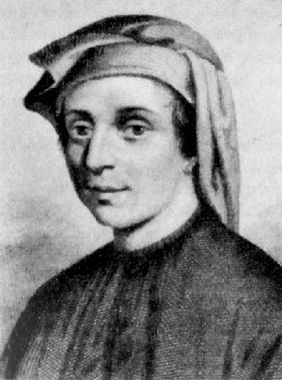
\includegraphics[width=2cm]{img/fibonacci}
\end{center}
La célèbre suite de Fibonacci, notée $F$, est définie ainsi :
\begin{itemize}
    \item   Ses deux premiers termes $F_0$ et $F_1$ valent 1;
    \item   On construit chaque terme suivant en faisant la somme des deux précédents.
\end{itemize}

De proche en proche, on calcule :
\begin{itemize}
    \item $F_2=1+1=2$
    \item  $F_3=2+1=3$
    \item $F_4=3+2=5$
    \item \textit{et c\ae tera}
\end{itemize}
Et plus généralement
$$F_n=\begin{cases}
        1               & \mbox{si } n=0\mbox{ ou }n=1 \\
        F_{n-1}+F_{n-2} & \mbox{sinon}
    \end{cases}$$


\begin{encadrecolore}{Pseudocode}{UGLiYellow}
    \begin{minted}{pseudocode}
        fonction fibonacci(n : entier naturel) -> entier naturel
            si n < 2 alors
                renvoyer 1
            sinon
                renvoyer fibonacci(n - 1) + fibonacci(n - 2)
            fin si
\end{minted}
\end{encadrecolore}

\begin{exercice}
    Programmer la fonction  \mintinline{python}{fibonacci} en \textsc{Python} et vérifier que  \mintinline{python}{fibonacci(30)} vaut \np{1346269}.
\end{exercice}


%

\subsection{Remarques}
\begin{itemize}
    \item La récursivité est un des concepts \textit{fondamentaux} de l'informatique.\\
          On dit que c'est un \textbf{paradigme de programmation}.
    \item Certains algorithmes se programment naturellement de manière récursive.
    \item Certaines \textbf{structures de données} se définissent également de manière récursive.
\end{itemize}


\section{La « magie» a un coût}



%

\subsection{La pile d'appels}


\picright{0.32}{img/appels}{

Que se passe-t-il réellement en machine lorsqu'on évalue la fonction récursive \mintinline{python}{factorielle(3)} ?\\

\textsc{Python} possède une \textbf{pile} : c'est une structure de données simple, qui permet d'empiler et de dépiler des données un peu comme on empile des assiettes.\\  

Lors de chaque appel récursif, une valeur est empilée en attendant le résultat de l'appel.

Lorsqu'il y a beaucoup d'appels récursifs \textit{imbriqués}, la taille de la pile augmente.\\
Pour éviter qu'elle sature, \textsc{Python} fixe la limite des appels récursifs \textit{imbriqués} à 999. Dès que l'on dépasse cette limite on obtient un message d'erreur :

\color{red} \texttt{\footnotesize RecursionError: maximum recursion depth exceeded in comparison}\color{black}
}
\newpage 
On peut fixer la taille de la pile Pour aller jusqu'à \np{10000} appels récursifs au maximum (par exemple).

\begin{pyc}
    \begin{minted}{python}
        import sys

        sys.setrecursionlimit(10_000)
    \end{minted}
\end{pyc}

\begin{exercice}
    Reprendre la fonction récursive \mintinline{python}{fibonacci} et utiliser le site \texttt{http://pythontutor.com/visualize.html} pour visualiser la pile d'appels lors de l'évaluation de \mintinline{python}{fibonacci(5)}.\\
    
    Quel commentaire peut-on faire ?
\end{exercice}


\section{Exercices}

\subsection*{Exercices de base}

\begin{encadrecolore}{Activité préparatoire}{UGLiOrange}
	Te rappelles-tu ce qu'est une poignée de main ? Voici comment \textsc{Wikipédia} définit cette coutume « pré-Covid 19 »:\\
	\textit{Une poignée de main est un geste de communication effectué le plus souvent en guise de salutation mais qui peut également être une signification de remerciement ou d'accord.}
	\begin{center}
		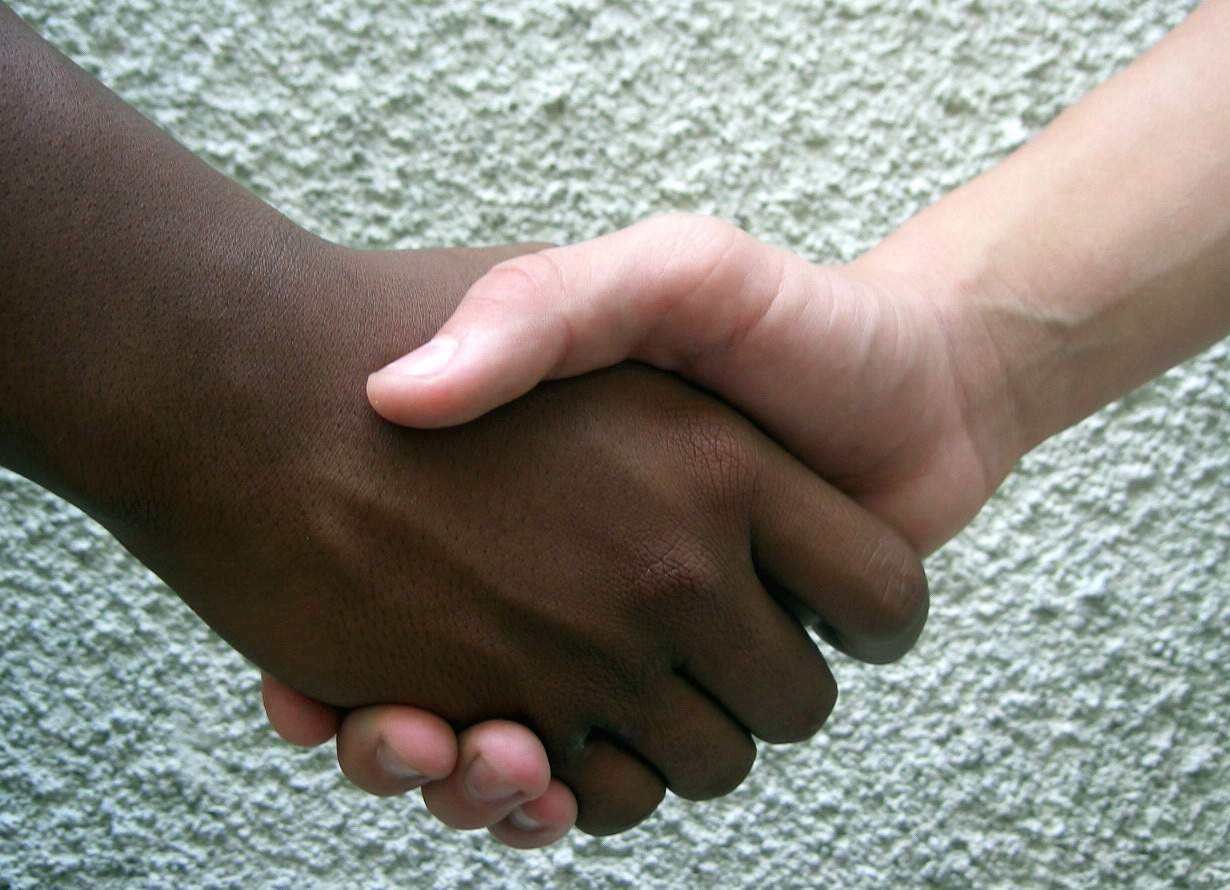
\includegraphics[width=3cm]{img/poignee.jpg}
	\end{center}
	On se pose la question suivante : « Quand $n$ personnes se rencontrent, si chacun serre la main des autres une seule fois, combien cela fait-il de poignées de main en tout ? ».\\
	On décide de noter $f(n)$ ce nombre.
	\begin{enumerate}
		\item 	\begin{enumalph}
			      \item 	Que valent $f(2)$, $f(3)$, $f(4)$, $f(5)$ ?
			      \item 	Que valent logiquement $f(1)$ et $f(0)$ ?
		      \end{enumalph}
		\item 	Supposons que l'on connaisse $f(10)$. Une 11\eme personne arrive. Combien doit-on ajouter à $f(10)$ pour obtenir $f(11)$ ?
		\item   Pour tout $n\in\N^*$, déduis-en ce que vaut $f(n)$ à partir de $f(n-1)$.
		\item   À partir du résultat précédent, écrit en \textsc{Python} la fonction \mintinline{python}{f} qui :
		      \begin{itemize}
			      \item 	en entrée prend un \mintinline{python}{int n} positif;
			      \item 	renvoie le nombre de poignées de mains lors de la rencontre de \mintinline{python}{n} individus.
		      \end{itemize}
		      \textbf{Indice :} rien n'interdit à \mintinline{python}{f} de «s'appeler elle-même» !
	\end{enumerate}
\end{encadrecolore}

\begin{exercice}[]
	En s'inspirant de la fonction factorielle, coder en \textsc{Python} de manière récursive la fonction \mintinline{python}{somme} qui
	\begin{itemize}
		\item 	en entrée prend un entier naturel \mintinline{python}{n};
		\item 	renvoie zéro si \mintinline{python}{n} vaut zéro;
		\item 	renvoie \mintinline{python}{n + somme(n - 1)} sinon.
	\end{itemize}
	On vérifiera que \mintinline{python}{somme(1000)} vaut \np{5050}. Expliquer ce que calcule \mintinline{python}{somme(n)}.
\end{exercice}

\begin{exercice}
	Programmer la fonction \mintinline{python}{sommes_cubes} en Python de manière récursive, et tester cette fonction.\\
	\mintinline{python}{sommes_cubes(n)} devra renvoyer, pour $n\in\N$ $$\sum_{k=0}^nk^3$$ C'est-à-dire la somme des cubes des entiers naturels de 0 à $n$.
\end{exercice}

\begin{exercice}[ : récursion imbriquée]
    \begin{center}
        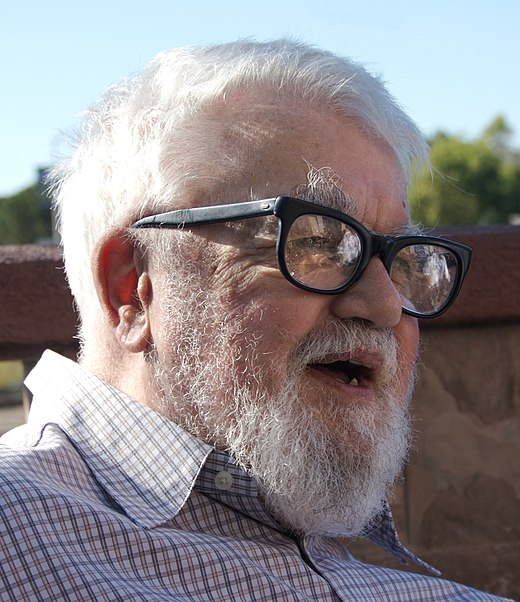
\includegraphics[width=4cm]{img/mccarthy}\\\scriptsize
        John McCarthy, informaticien, lauréat du prix Turing en 1971.
    \end{center}
		La fonction $f_{91}$ de McCarthy est définie sur $\N$ par :
		$$f_{91}(n)=\begin{cases}
				n-10                            & \mbox{si } n>100 \\
				f_{91}\left(f_{91}(n+11)\right) & \mbox{sinon}
			\end{cases}$$
		Programmer $f_{91}$ en \textsc{Python} et vérifier que pour tout entier naturel $n$ inférieur ou égal à 101, $f_{91}(n)$ vaut... 91.


\end{exercice}

\begin{exercice}[ : fonction puissance]
	Coder en \textsc{Python} la fonction \mintinline{python}{puissance} qui
	\begin{itemize}
		\item 	en entrée prend un \mintinline{python}{int} positif \mintinline{python}{n} et un \mintinline{python}{float x};
		\item 	renvoie la valeur de \mintinline{python}{x**n} calculée récursivement (cas de base et cas récursif à trouver soi-même).
	\end{itemize}
\end{exercice}


\begin{exercice}[ : récursion mutuelle]
	On considère les deux suites $a$ et $b$ définie par
	$$a(n)=\begin{cases}
			1           & \mbox{si } n=0 \\
			n-b(a(n-1)) & \mbox{sinon}
		\end{cases}
		\mbox{\hspace{3em} et\hspace{3em}}
		b(n)=\begin{cases}
			0           & \mbox{si } n=0 \\
			n-a(b(n-1)) & \mbox{sinon}
		\end{cases}$$
	
	Programmer $a$ et $b$ en \textsc{Python}, puis conjecturer pour quelles valeurs de $n$ on a $a(n)\neq b(n)$ (ces valeurs sont en relation avec une suite déjà rencontrée).
\end{exercice}


\begin{exercice}[ : palindromes]
	Un \mintinline{python}{str} est un palindrome si on peut le lire à l'envers comme à l'endroit. Par exemple « kayak», «  Un radar nu » ou « !a!bcb!a!» sont des palindromes.\\
	\'Ecrire une fonction récursive \texttt{palindrome} qui :
	\begin{itemize}
		\item 	en entrée prend un mot (un \mintinline{python}{str});
		\item 	renvoie \mintinline{python}{True} si c'est un palindrome et \mintinline{python}{False} sinon;
		\item 	procède récursivement
		      \begin{itemize}
			      \item 	si le mot a une lettre ou bien deux lettres pareilles, c'est un palindrome;
			      \item 	sinon on regarde si les lettres du début et de la fin sont les mêmes. Si ce n'est pas le cas, ce n'est pas un palindrome. Si c'est le cas alors il faut regarder si le sous-mot restant est un palindrome.
		      \end{itemize}
	\end{itemize}
	\textbf{Rappels :}
	Si \mintinline{python}{s} est un \mintinline{python}{str}
	\begin{itemize}
		\item 	\mintinline{python}{s[0]} et \mintinline{python}{s[-1]} sont respectivement son premier caractère et son dernier caractère.
		\item 	\mintinline{python}{s[p:q]} renvoie la sous chaîne allant de \mintinline{python}{s[p]} à \mintinline{python}{s[q-1]}.
	\end{itemize}
\end{exercice}


\subsection*{Avec de l'arithmétique}
\begin{definition}[ : division euclidienne dans \N]
	
	Soient A et B deux entiers naturels, et $B\neq 0$. Il existe deux nombres uniques Q et R (vérifiant $0\leqslant R<B$) tels que l'on puisse écrire
	$$A = Q\times B + R$$
	
	C'est exactement la division que l'on a apprise à l'école primaire (celle où l'on s'arrête aux nombres entiers):
	\begin{center}
		\begin{tabular}{r|l}
			A & B \\
			\cline{2-2}
			R & Q
		\end{tabular}
		
		\begin{itemize}
			\item 	A est appelé le \textit{dividende} ;
			\item 	B est le \textit{diviseur} ;
			\item	Q est le \textit{quotient} ;
			\item 	R est le \textit{reste}, il est \textit{impérativement} plus petit que B.
		\end{itemize}
	\end{center}
\end{definition}

En \textsc{Python} on obtient \mintinline{python}{Q} en évaluant \mintinline{python}{A // B} et \mintinline{python}{R} en évaluant \mintinline{python}{A % B}, cette dernière opération se lit « \mintinline{python}{A} modulo \mintinline{python}{B}».Voici un exemple

\begin{pyc}
	\begin{minted}{python}
>>> 22 // 7
3
>>> 22 % 7
1
\end{minted}
\end{pyc}


\begin{exercice}[]
	\begin{enumerate}
		\item 	En \textsc{Python}, écrire une fonction \mintinline{python}{units_digit} qui
		      \begin{itemize}
			      \item 	en entrée prend un \mintinline{python}{int} positif ;
			      \item 	renvoie un \mintinline{python}{int} qui est son chiffre des unités.
		      \end{itemize}
		\item 	De même écrire une fonction \mintinline{python}{hundreds_digit} pour le chiffre des centaines.
		\item 	De même pour une fonction \mintinline{python}{thousands_digit} qui renvoie le chiffre des milliers.
	\end{enumerate}
\end{exercice}

\begin{exercice}[]
	\'Ecrire une fonction récursive \mintinline{python}{decimal_length}  basée sur \mintinline{python}{//} et/ou  \mintinline{python} qui
	\begin{itemize}
		\item 	en entrée prend un \mintinline{python}{int} positif ;
		\item 	renvoie un \mintinline{python}{int} qui est le nombre de chiffres de l'écriture binaire de ce nombre.
	\end{itemize}
\end{exercice}


\begin{exercice}[]
	On considère le procédé suivant :
	\begin{itemize}
		\item 	soit $m\in \N$ un entier écrit en écriture décimale $m = (a_p\cdots a_1a_0)_{10}$,\\
		      par exemple $m=\np{31976}$;\\
		\item 	on « coupe» cette écriture en deux au niveau des unités : avec $m$ on forme $m_1=(a_p\cdots a_1)_{10}$ et $m_2=(a_0)_{10}$,\\
		      pour notre exemple $m_1=\np{3197}$ et $m_2=6$;\\
		\item	On calcule  $m'=m_1-2m_2$ ,\\
		      pour notre exemple cela donne $m'=\np{3197}-2\times 6 = 3185$\\
	\end{itemize}
	
	\begin{enumerate}
		\item 	à l'aide de \mintinline{python}{//} et/ou  \mintinline{python}{%} écrire une fonction \mintinline{python}{f} qui
		      \begin{itemize}
			      \item 	en entrée prend un \mintinline{python}{int} positif \mintinline{python}{m} ;
			      \item 	en sortie renvoie \mintinline{python}{m'}.
		      \end{itemize}
		\item 	En fait, la fonction $f$ donne un critère de divisibilité par 7 pour un entier $m$ :
		      \begin{itemize}
			      \item 	si  $m\leqslant 70$ alors s'il appartient à {-7; 0; 7; 14; 21; 28; 35; 42; 49; 56; 63; 70}, $m$ est divisible par 7, sinon il ne l'est pas ;
			      \item 	sinon on regarde si $f(m)$ est divisible par 7.
		      \end{itemize}
		      Pour notre exemple on obtient $$31\,976 \mapsto 3\,197 - 2\times 6 = 3\, 185 \mapsto 318- 2\times 5 =308 \mapsto 30 - 2\times 8= 14$$ et on en conclut qu'il est divisible par 7.\\
		      
		      Programmer une fonction récursive \mintinline{python}{is_divisible_by_7} qui
		      \begin{itemize}
			      \item 	en entrée prend un \mintinline{python}{int} positif ;
			      \item 	en sortie renvoie \mintinline{python}{True} ou \mintinline{python}{False} selon que l'entier est divisible par 7.
		      \end{itemize}
		      Cette fonction utilisera la fonction \mintinline{python}{f} définie précédemment.
	\end{enumerate}
\end{exercice}

\begin{exercice}[ : algorithme d'Euclide récursif]
	Soient $n$ et $p$ deux entiers strictement positifs. On note $\mbox{pgcd}(a;b)$ le plus grand entier qui divise à la fois $a$ et $b$.\\
	Par exemple
	\begin{itemize}
		\item 	$1050 = 2\times 3\times	5\times 5\times 7$;
		\item 	$770=2\times 5\times 7\times 11$;
		\item 	le pgcd de ces deux nombres est donc $2\times 5\times 7 =70$.
	\end{itemize}
	Pour trouver le pgcd de deux nombres on peut, comme dans l'exemple précédent, les décomposer en produit de facteurs premiers et prendre le produit de tous les facteurs communs, mais on peut aussi utiliser l'algorithme d'Euclide :\\
	Soient $a$ et $b$ deux entiers strictement positifs, on suppose que $a\leqslant b$
	\begin{enumerate}
		\item on écrit la division euclidienne de $a$ par $b$ : $a=q\times b + r$ avec $r<b$;
		\item si un entier divise $a$ et $b$ alors on peut facilement montrer qu'il divise aussi $r$, de sorte que $\mbox{pgcd}(a;b)=\mbox{pgcd}(b;r)$.
		\item si $r\neq 0$ alors on recommence alors en prenant $a$ égal à $b$ et $b$ égal à $r$;
		\item si $r=0$ alors le pgcd des nombres de départ est le dernier $b$ qu'on a utilisé.
	\end{enumerate}
	Voyons la méthode sur un exemple :
	\begin{itemize}
		\item 	on divise $1050$ par $280$ : $1050 = 1\times 770 + 280$
		\item 	on divise $770$ par $280$ : $770 = 2\times 280 + 210$
		\item 	on divise $280$ par $210$ : $280 = 1\times 210 + 70$
		\item 	on divise $210$ par $70$ : $210 = 3\times 70 + 0$
		\item 	le reste est nul, le dernier diviseur est 70 et c'est le pgcd des deux nombres de départ.
	\end{itemize}
	Programmer cette fonction \mintinline{python}{pgcd} de manière récursive.
\end{exercice}

\subsection*{À savoir faire absolument}
\begin{exercice}[ : lire un code]
	On considère la fonction suivante :
	
	
	\begin{minted}{python}
def mystery3(lst: list) -> bool:
    """lst est une liste d'int non vide"""
    if len(lst) > 1:
        if lst[0] > lst[1]:
            return False
        else:
            return mystery3(lst[1:])
            # on rappelle que lst[1:] désigne la liste composée
            # de lst[1],lst[2], etc jusqu'au dernier élément de lst
    else:
        return True
\end{minted}
	
	
	\begin{enumerate}
		\item Calculer \mintinline{python}{mystery3([5])} ;
		\item Calculer \mintinline{python}{mystery3([5, 7])} ;
		\item Calculer \mintinline{python}{mystery3([5, 1])} ;
		\item Calculer \mintinline{python}{mystery3([5, 10, 8])} ;
		\item Que fait donc cette fonction ?
	\end{enumerate}
\end{exercice}
\begin{exercice}[ : produire un code récursif]
	
	\begin{enumerate}
		\item \'Ecrire une fonction récursive \mintinline{python}{maxi} qui
		      \begin{itemize}
			      \item en entrée prend une liste d' \mintinline{python}{int} ;
			      \item renvoie le maximum de cette liste.
		      \end{itemize}
		      Vous pouvez utiliser la fonction \mintinline{python}{max}.
		\item \'Ecrire une fonction récursive \mintinline{python}{reverse} qui
		      \begin{itemize}
			      \item en entrée prend un \mintinline{python}{str} ;
			      \item renvoie ce \mintinline{python}{str} « à l'envers »
		      \end{itemize}
		      Par exemple, \mintinline{python}{reverse("salut")} devra renvoyer \mintinline{python}{"tulas"}.
	\end{enumerate}
\end{exercice}
\newpage 
\subsection*{Excercices supplémentaires}

\begin{exercice}[* : nombres de Catalan]


		Considérons l'opération « puissance». appliquée à trois nombres, par exemple 2, 3 et 4, pris dans cet ordre. Il y a plusieurs manière de
		procéder :
		\begin{itemize}
			\item	$2^{(3^4)}=2^{81}=2 417 851 639 229 258 349 412 352$
			\item 	$(2^3)^4 = 8^4=4096$
		\end{itemize}
		Pour 3 nombres, il y a donc 2 manières de placer les parenthèses pour effectuer les opérations.\\
		Et pour 4 nombres ? Pour 5 ?
		Pour simplifier l’écriture on peut noter $a*b$ au lieu de $a^b$. \\
		Alors avec $n$ lettres on peut reformuler l’exemple précédent ainsi
		: quel est le nombre de manières (noté $C_n$) de placer des parenthèses autour des lettres de sorte que

		\begin{center}
			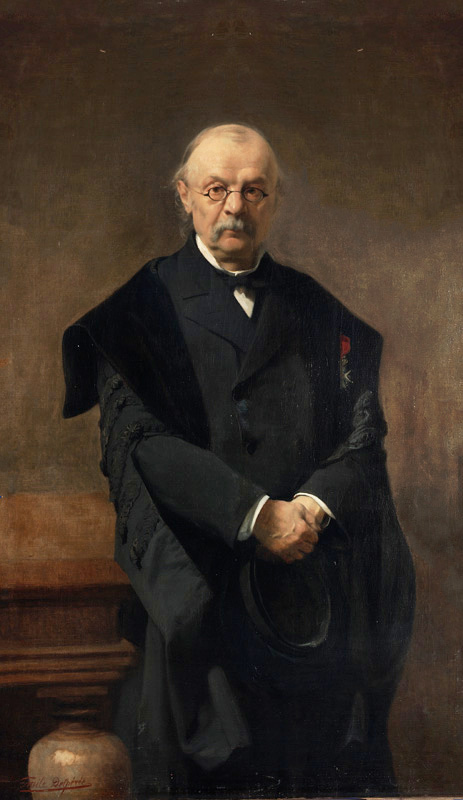
\includegraphics[width=4cm]{img/catalan}\\\scriptsize
			Eugène Catalan, mathématicien franco-belge du \textsc{xix}\eme siècle.
		\end{center}
	
	\begin{itemize}
		\item 	on n'ait jamais plus de deux termes non parenthésés : pas de choix à faire ;
		\item 	on ne mette jamais des parenthèses autour d’un seul terme : pas de parenthèses inutiles.
	\end{itemize}
	Les premiers cas sont simples :
	
	\begin{itemize}
		\item 	$C_1=1$ : il n'y a qu'une manière d'écrire $a$.
		\item 	$C_2=1$ aussi : une seule possibilité : $a*b$.
		\item 	$C_3=2$, on l'a vu : $a*(b*c)$ et $(a*b)*c$.
		\item 	Pour calculer $C_4$, on peut classer les parenthésages suivant la dernière opération $*$ à faire :
		      \begin{itemize}
			      \item 	après $a$ : il y a $a*((b*c)*d)$ et $a*(b*(c*d))$.
			      \item 	« entre $b$ et $c$» : $(a*b)*(c*d)$.
			      \item 	juste avant $d$ : $((a*b)*c)*d$ et $(a*(b*c))*d$.
		      \end{itemize}
		      Finalement cela fait 5 possibilités, $C_4=5$ et on remarque que $C_4=C_1C_3+C_2C_2+C_3C_1$.
	\end{itemize}
	Cela se généralise : pour tout $n$ entier supérieur à 2 on a
	$$C_n=C_1C_{n-1}+C_2C_{n-2}+\ldots+C_{n-1}C_1$$
	En effet, on commence par choisir la position de la dernière opération à effectuer : puisqu'il y a $n$ lettres il y a $n-1$ choix de positions
	possibles, chacun scindant le mot de $n$ lettres en un mot de $p$ lettres et un autre de $n-p$, qui donnent donc lieu respectivement à $C_p$ et
	$C_{n-p}$ parenthésages indépendants, donc $C_pC_{n-p}$ parenthésages en tout. En considérant toutes les valeurs de $p$ possibles on arrive à
	\begin{equation}
		\tag{*}
		C_n=\sum_{p=1}^{n-1}C_pC_{n-p}
		\label{eqn:Catalan}
	\end{equation}
	
	Ce qui permet de calculer $C_5 =14$, $C_6 =42$, $C_7 =132$, $C_8 =429$, $C_9 =1430$, $C_{10} =4862$...\\
	
	\textbf{Travail à faire :}\\
	
	Programmer la fonction \mintinline{python}{catalan} en \textsc{Python} :
	\begin{itemize}
		\item 	Le cas de base est pour \mintinline{python}{n} valant \mintinline{python}{1}, où la fonction renvoie \mintinline{python}{1};
		\item 	Si \mintinline{python}{n} est plus grand, alors on calcule \mintinline{python}{catalan(n)} récursivement à l'aide de \eqref{eqn:Catalan}.
	\end{itemize}
	
	On pourra utiliser la fonction \texttt{sum}.\\
	Par exemple \mintinline{python}{sum(n for n in range(10))} calcule la somme $0+1+...+9$.
\end{exercice}


\begin{exercice}[* : approximation d'un flocon de Von Koch]
	On part d'un segment (étape 0) que l'on coupe en 3 parties égales. Sur le segment du milieu on construit un triangle équilatéral puis on enlève ce segment. On obtient alors une itération du procédé de Von Koch. On peut ensuite répéter indéfiniment ce procédé.
	\begin{center}
		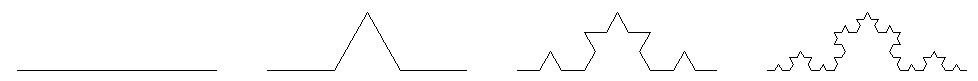
\includegraphics[width=\linewidth]{img/koch}\\
		\scriptsize Les 4 premières étapes du procédé.
	\end{center}
	Lorsque l'on part d'un triangle équilatéral auquel on applique ce procédé une infinité de fois, l'objet obtenu s'appelle un \textit{flocon de Von Koch}. Il a la particularité d'avoir une aire finie mais un périmètre infini.
	\begin{center}
		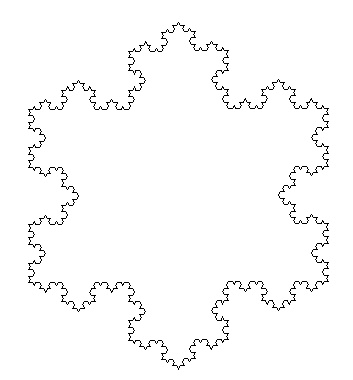
\includegraphics[width=6cm]{img/flocon}\\
		\scriptsize Une approximation d'un flocon de Von Koch.
	\end{center}
	Pour dessiner, on va utiliser le module \mintinline{python}{turtle} de \textsc{Python}.
	\begin{enumerate}
		\item  Regarde bien le micro-tutoriel pour comprendre le fonctionnement de base de \mintinline{python}{turtle}.
		\item 	Coder la fonction \mintinline{python}{koch} qui
		      \begin{itemize}
			      \item 	en entrée prend un \mintinline{python}{float x} (longueur du segment de base) et un \mintinline{python}{int n} (nombre d'itérations);
			      \item 	ne renvoie aucune valeur mais dessine le processus itéré n fois, de manière récursive.
		      \end{itemize}
	\end{enumerate}
\end{exercice}

\begin{exercice}[* : fonction puissance améliorée]
	Soit $x$ un nombre réel et $n$ un entier positif alors on a \\
	$$x^n=\begin{cases}
			(x^{n/2})^2            & \mbox{si } n \mbox{ est pair} \\
			x\times(x^{(n-1)/2})^2 & \mbox{sinon}
		\end{cases}$$
	\begin{enumerate}
		\item 	En se basant sur cette observation, coder une fonction \mintinline{python}{puissance_amelioree} qui a les mêmes spécifications que la fonction \mintinline{python}{puissance} vue dans un exercice précédent.
		\item 	Créer pour ces deux fonctions une variable \mintinline{python}{nb_appels} pour comptabiliser le nombre d'appels récursifs et comparer ces nombres dans \mintinline{python}{puissance(2,128)} et \mintinline{python}{puissance_amelioree(2,128)}.
	\end{enumerate}
\end{exercice}
\end{document}